\textcolor{black}{\section{Resultados y Análisis}}

\subsection{PARTE 1}
\noindent Al graficar el campo eléctrico reducido contra velocidad de deriva  se obtuvieron las siguientes graficas que se muestran en la Figura \ref{Graf:Graficas}
 
 \begin{figure}%[H]
 	\centering
 	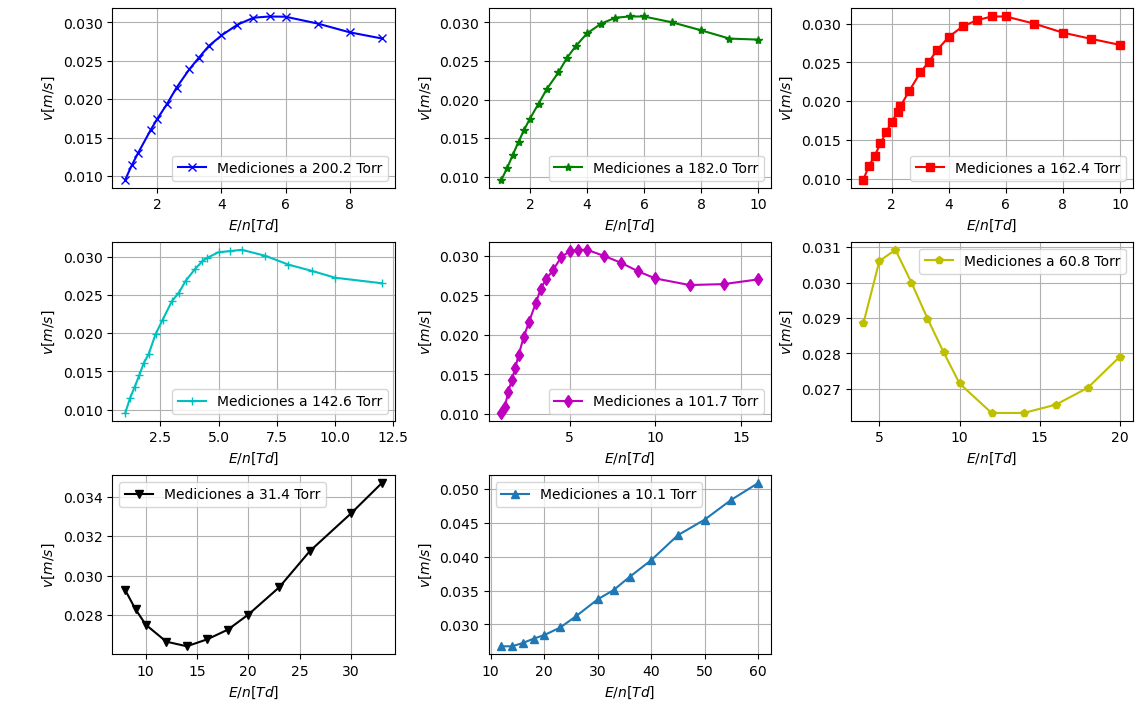
\includegraphics[scale=0.35]{figs/Graficas.png}
 	\caption{Gráficas de campo eléctrico reducido contra velocidad de deriva a diferentes presiones}
 	\label{Graf:Graficas}
 \end{figure}
 
 Como podemos ver a medida que la presión va disminuyendo podíamos suministrar un $E/N$ mayor sin que se produzcan descargas que dañen el equipo, esto se debe porque a presiones altas el voltaje necesario para crear el campo reducido supera el umbral de ruptura dieléctrica del gas creando chispas entre los electrodos, en cambio para bajas presiones era más fácil aplicar los campos si que el gas se ionizara.
 
 De las primeras cinco graficas que se muestran en la figura \ref{Graf:Graficas}, podemos observar que existe un rápido crecimiento de $v_d$ entre 1 y 5 Td. Esto se debe a que en esta sección los electrones ganan energía y se acercan al mínimo de Ramsauer-Townsend dejando de chocar disparando si su velocidad de deriva.
 
 Después si analizamos las graficas de $101.7Torr$ y $60.8Torr$ una vez que llega a la máxima velocidad podemos ver que comienza a bajar conforme aumenta $E/N$, esto se debe a que en esta parte comienza la interacción con el $N_2$ que tiene niveles de vibración que absorben la energía en este rango, entonces los electrones pierden su energía y vuelven a colisionar con el argón. Este efecto se conoce como \textcolor{black}{Conductividad Diferencial Negativa}.
 
 Finalmente en las graficas de $31.4Torr$ y $10.1Torr$ podemos apreciar que la velocidad vuelve a subir esto se debe a que $E/N$ es muy alto y los electrones ganan tanta energía que la que pierden en vibración se vuelve despreciable, así como también que la sección eficaz de colisión vuelve a bajar porque la energía cinética promedio es muy alta.
 
 Además se esbozó una gráfica donde se sobreponen todas las gráficas que se muestran en la figura \ref{Graf:Graficas}, dicha grafica se muestra en la Figura \ref{Graf:Quimera}
  \begin{figure}%[H]
 	\centering
 	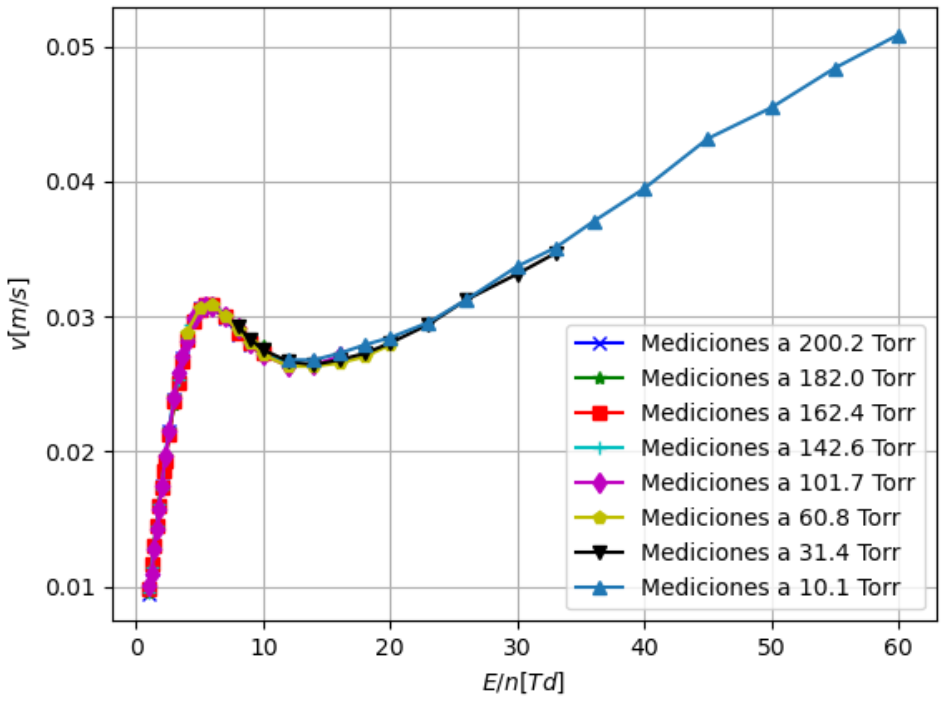
\includegraphics[scale=0.4]{figs/Quimera.png}
 	\caption{Gráfica creada al sobreponer el comportamiento a diferentes presiones de $E/N$ vs $v_d$ }
 	\label{Graf:Quimera}
 \end{figure}
 
 
\subsection{PARTE 2}
\noindent Con las mediciones hechas de forma manual se obtuvieron las gráficas de las Figuras \ref{Graf:2v_manual}, \ref{Graf:3v_manual} y \ref{Graf:4v_manual}.

\begin{figure}%[H]
	\centering
	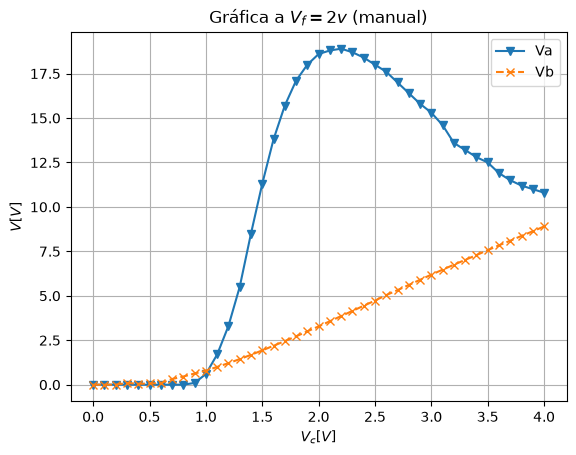
\includegraphics[scale=0.4]{figs/part2-2v_manual.png}
	\caption{Gráfica del voltaje del ánodo y del voltaje de la rejilla-blindaje registradas por el multímetro  contra el voltaje del cátodo a un voltaje fuente de $2\,V$.}
	\label{Graf:2v_manual}
\end{figure}

\begin{figure}%[H]
	\centering
	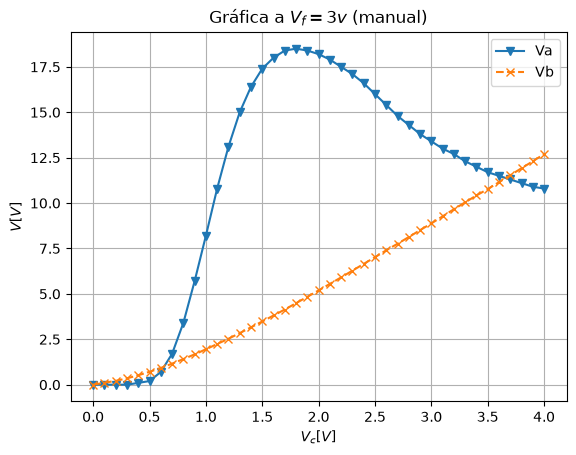
\includegraphics[scale=0.4]{figs/part2-3v_manual.png}
	\caption{Gráfica del voltaje del ánodo y del voltaje de la rejilla-blindaje registradas por el multímetro  contra el voltaje del cátodo a un voltaje fuente de $3\,V$.}
	\label{Graf:3v_manual}
\end{figure}

\begin{figure}%[H]
	\centering
	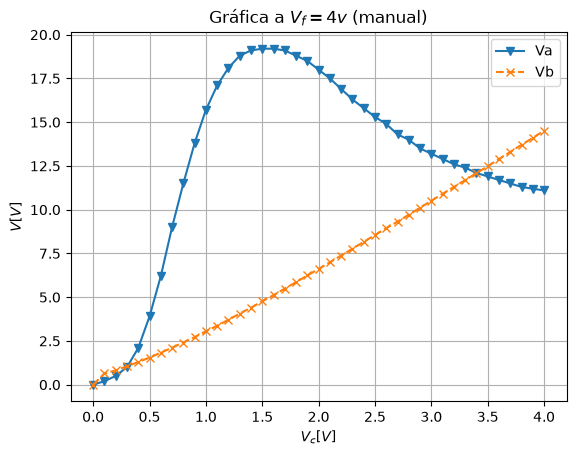
\includegraphics[scale=0.4]{figs/part2-4v_manual.png}
	\caption{Gráfica del voltaje del ánodo y del voltaje de la rejilla-blindaje registradas por el multímetro  contra el voltaje del cátodo a un voltaje fuente de $4\,V$.}
	\label{Graf:4v_manual}
\end{figure}

Como podemos ver de las gráficas  \ref{Graf:2v_manual}, \ref{Graf:3v_manual} y \ref{Graf:4v_manual} existe una tendencia de $V_a$ de aumentar rápidamente y posteriormente desciende gradualmente, esto se debe a que $V_c$ define la energía cinética con la que los electrones atraviesan el gas, por lo que existe una sección de mínima dispersión, y una vez que se llegar a al máximo de la sección eficaz es tanta la energía cinética de los electrones que aumenta las colisiones de estos por lo cual disminuye de nuevo.

También podemos observar que al cambiar $V_f$ la sección eficaz  se recorre a la izquierda esto se debe a que si aumentas $V_f$ los electrones salen con mayor energía por eso necesitan menor $V_c$, también se debe a que se crea un nube de electrones en el cátodo, la cual crea su propio potencial eléctrico que acelera a los electrones, entonces si se aumenta el $V_d$ también aumenta la nube de electrones.

Las gráficas realizadas de las mediciones hechas por el software del laboratorio se pueden observar en las Figuras \ref{Graf:2v_automatic}, \ref{Graf:3v_automatic} y \ref{Graf:4v_automatic}.

\begin{figure}%[H]
	\centering
	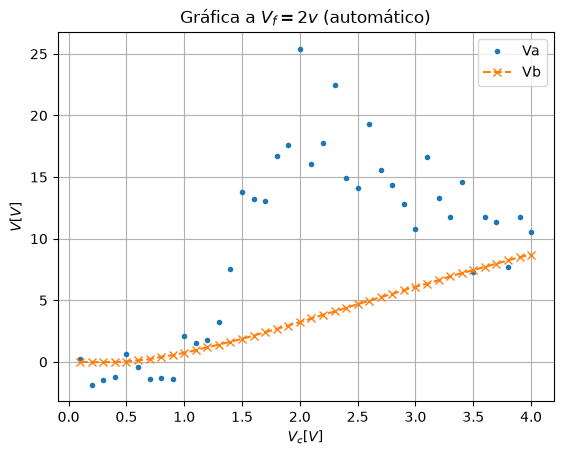
\includegraphics[scale=0.4]{figs/part2-2v_automat.png}
	\caption{Gráfica del voltaje del ánodo y del voltaje de la rejilla-blindaje registradas por el software del laboratorio contra el voltaje del cátodo a un voltaje fuente de $2\,V$.}
	\label{Graf:2v_automatic}
\end{figure}

\begin{figure}%[H]
	\centering
	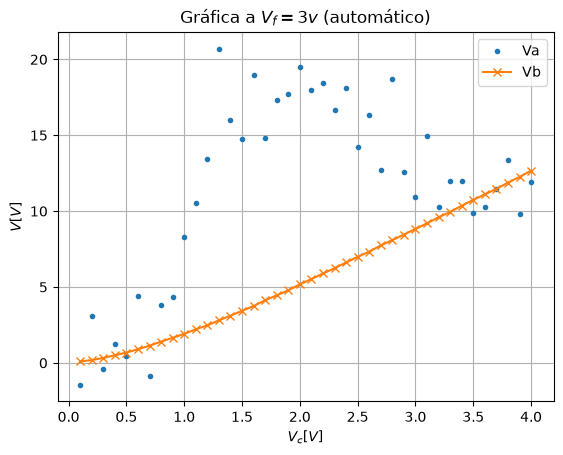
\includegraphics[scale=0.4]{figs/part2-3v_automat.png}
	\caption{Gráfica del voltaje del ánodo y del voltaje de la rejilla-blindaje registradas por el software del laboratorio contra el voltaje del cátodo a un voltaje fuente de $3\,V$.}
	\label{Graf:3v_automatic}
\end{figure}

\begin{figure}%[H]
	\centering
	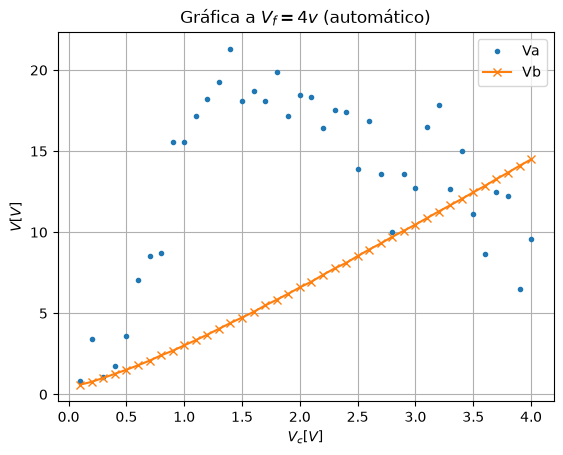
\includegraphics[scale=0.4]{figs/part2-4v_automat.png}
	\caption{Gráfica del voltaje del ánodo y del voltaje de la rejilla-blindaje registradas por el software del laboratorio contra el voltaje del cátodo a un voltaje fuente de $4\,V$.}
	\label{Graf:4v_automatic}
\end{figure}

Al observar los dato obtenidos de manera automática, podemos ver de las gráficas \ref{Graf:2v_automatic}, \ref{Graf:3v_automatic} y \ref{Graf:4v_automatic}, que existe una gran dispersión en el $V_a$ esto se debe a que el software tomó los datos al instante después de cambiar el $V_c$ y no espera a que el voltaje de diodo se estabilizara.  
